In this chapter planning and work-flow regarding Sprint 3 will be described. 
All from setting our goals to implementation and testing. On the end we will evaluate whole sprint and try to answer on following questions: What went well? What could be improved? What should we start doing?  
% TODO rewrite

\section{Sprint planning}
In the planning part of sprint 2 when there have been introduced and idea or goal for refining and extent the existing code, customer agreed, with condition, that sprint 3 will be focused on image processing part.

As the image processing module was one of the major risks, there was done some preliminary studies research even in the end of sprint 2 about possible approaches.
One specific way to deal with the problem (using OpenCV and Hough Transformation\footnote{http://docs.opencv.org/doc/tutorials/imgproc/imgtrans/hough\_lines/hough\_lines.html}) was introduced to customer in planning part of meeting.
Customer was not satisfied with such a low-level approach and wanted us to use some existing tools.
Therefore there was need for additional preliminary studies concerning existing projects or libraries that could be used.
You can read more about additional preliminary studies below.

This time there was made an proposal of additional "pre-demo" video showing the progress of implementation on Thursday 4 October 2013 during the regular meeting and customer gladly accepted this offer.


\subsection{Duration}
This sprint is 2 weeks long. From 30th September 2013 to 13th October 2013.
We agreed on the date of presentation and showing the running demo -- on Thursday 11 October 2013.
Estimated velocity is 240 hours since we agreed on 30 working hours per person per week.

\subsection{User-stories}

\subsubsection*{Implementation}
All the functional requirements for sprint 3 are presented in Table \ref{tab:sprint3stories}
\LTXtable{\textwidth}{sprint3/stories.tex}

\subsubsection*{Documentation}
All the documentation stories for sprint 3 are presented in Table \ref{tab:sprint3Documentationstories}
\LTXtable{\textwidth}{sprint3/storiesDocumentation.tex}

\subsubsection*{Project management}
All the project management for sprint 3 are presented in Table \ref{tab:sprint3storiesProcess}
\LTXtable{\textwidth}{sprint3/storiesProcess.tex}

\section{Preliminary studies}
% TODO

\section{Sprint goal}
The goal of this sprint is having a working application on a mobile phone that can work in two modes.  
Input type and output are for both modes common -- input is an image or video and output is location of detected mobile phones in a given matrix (e.g. 4x4 matrix) with color that mobile's screen is lighting.
In the first mode, real video from mobile's camera will be treated as an input and on the other hand in the second mode mock data (image or video) are treated as an input.

You can see example of input with matrix 2x2 in Figure \ref{img:sprint3_goal}. Appropriate output of image processing and mapping module is: \texttt{\{blue,[0,0]\}, \{red,[1,0]\}, \{green,[0,1]\}}.

\begin{figure}[H]
	\centering
		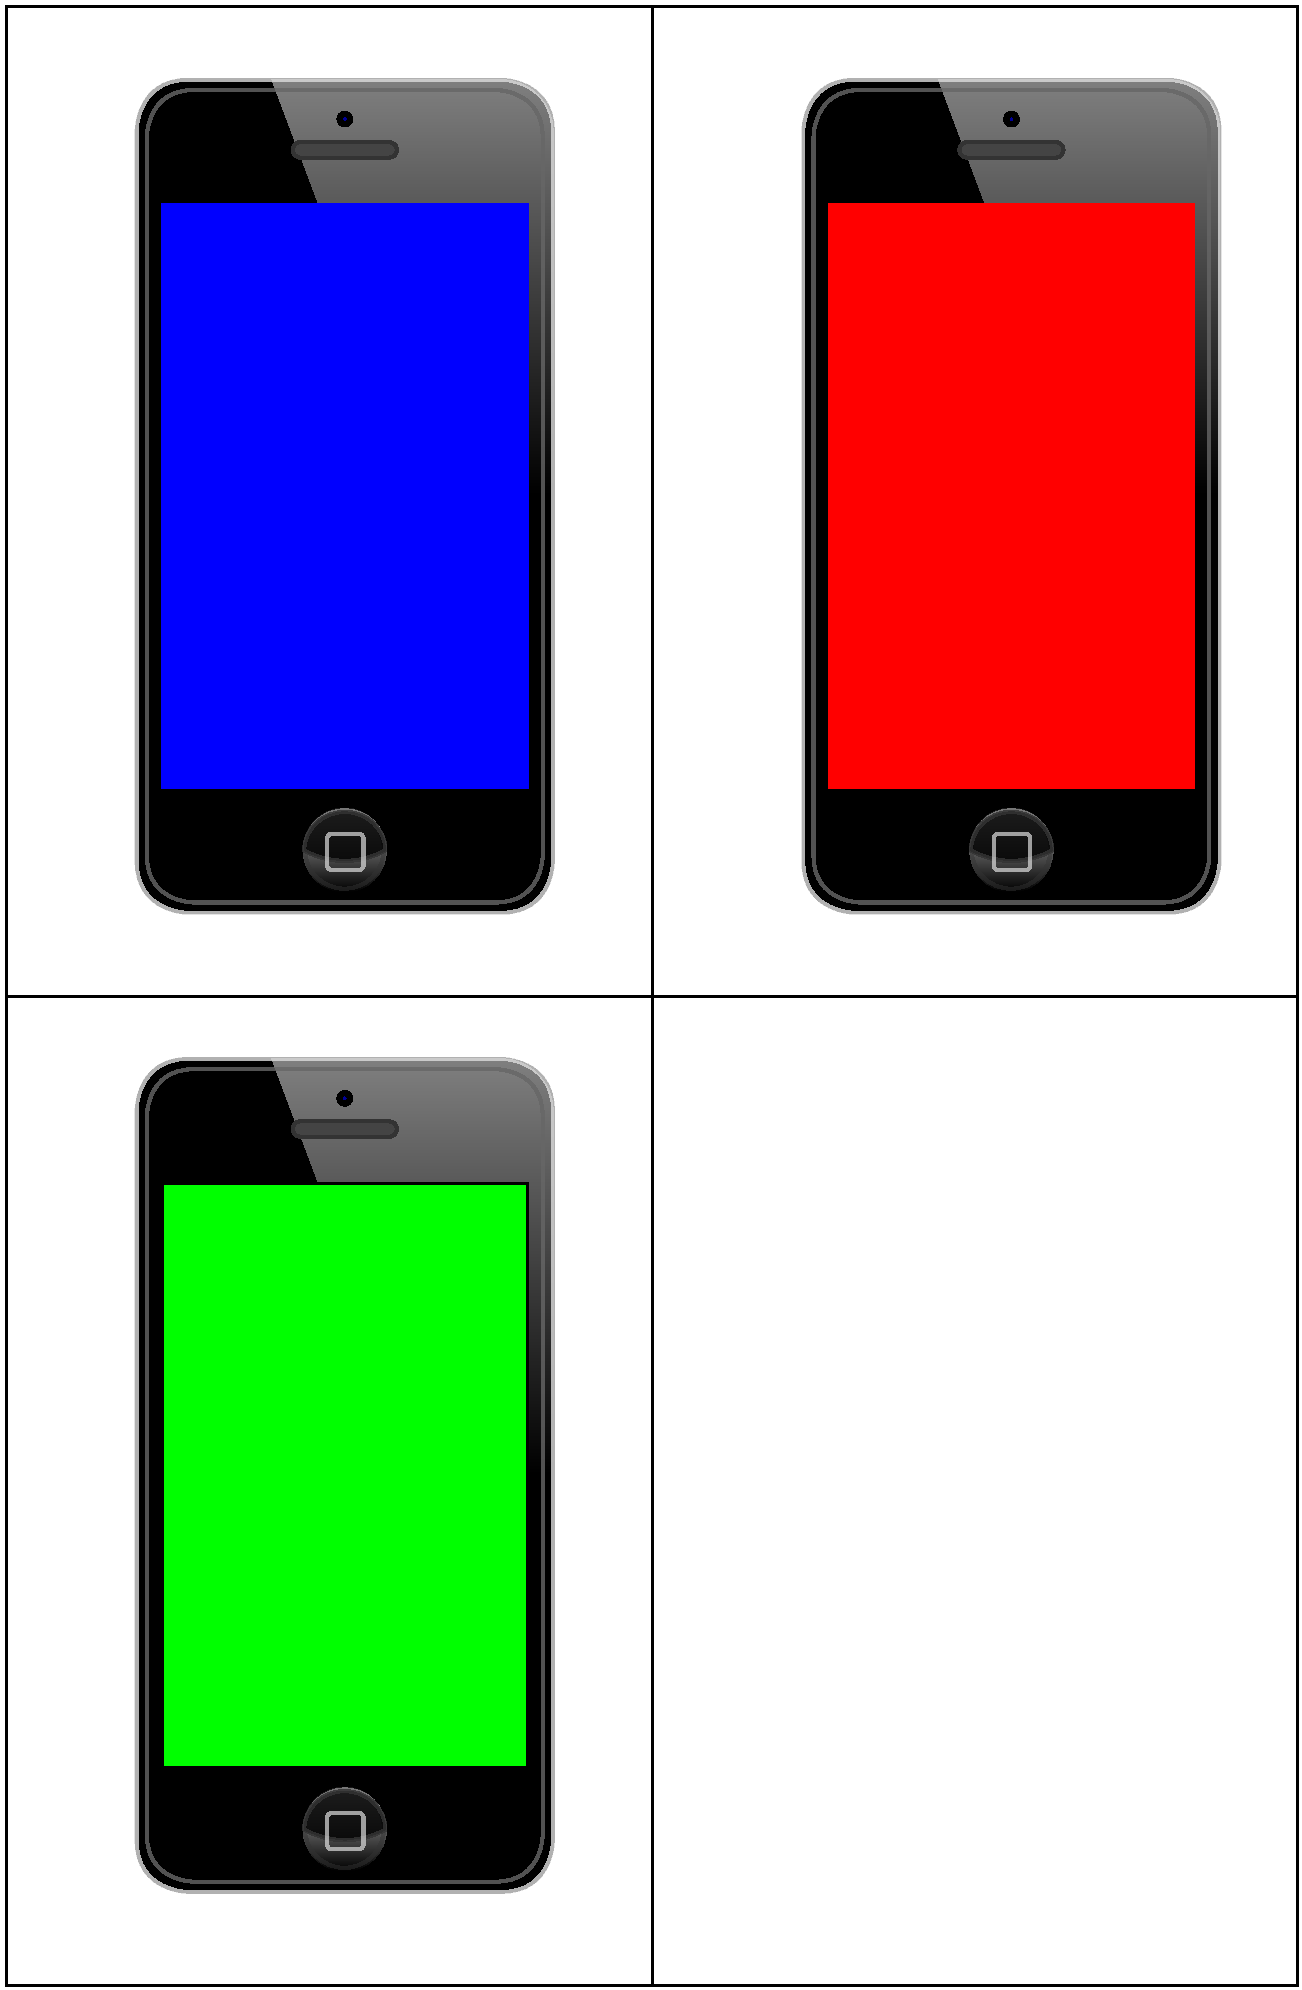
\includegraphics[width=7cm]{sprint3/sprint3_goal.pdf}
	\caption{Example of ideal data input for image processing module with 2x2 matrix.}
	\label{img:sprint3_goal}
\end{figure}


\section{Architecture}
In this section will be described image processing module using 4+1 architectural view module.

\subsection{Logical view}
You can see a class diagram of new classes created in sprint 3 in Figure \ref{fig:class_diagram_sprint3}. We can divide these new classes into three categories. 

Into the first category we count classes \texttt{LightDetector}, \texttt{TileMapper} and \texttt{PointCollector}. 
These classes are a core of image processing module. 
The only visible method for working with this module is \texttt{PointCollector}'s method \texttt{collect}.
This function accepts two parameters: first is the image where mobile phone's screen detection should be done and second is a list of colors of screens which should be detected. 
Method \texttt{collect} is run asynchronously (as a new thread due to possible high time demanding operations) and therefore it was designed as a design pattern \texttt{Observer}
As class \texttt{PointCollector} implements interface \texttt{Observable} (also known as a \emph{Subject} \cite[p.~326]{Gamma:1995:DPE:186897}), its \texttt{Observers} must implement method \texttt{update}. 
To this function is passed as a argument hash map with keys as a colors and values as a lists of tile positions with appropriate color.
Class \texttt{LightDetector} is responsible for detecting location of color blobs in given image. 
Results as a list of pixel's position of blobs are passed as a return value of function \texttt{getBlobCoords}. 
These values are fetched by instance of \texttt{PointCollector} and passed to \texttt{TileMapper}, which is responsible for mapping points into appropriate tiles in grid.

In second category there is only class \texttt{CameraActivity}, who is responsible for handling outputs from camera or mock device and also gives appropriate feedback on screen of mobile (draws grid and marks detected blobs).

In last category there is class \texttt{ColorManager}, which is standalone class and in application there is only need for one instance. Therefore it was designed as a \texttt{Singleton} pattern \cite[p.~144]{Gamma:1995:DPE:186897}. Its main purpose is to handle transformations of different color formats such as special library, network and internal formats.

\begin{figure}[H]
	\centering
		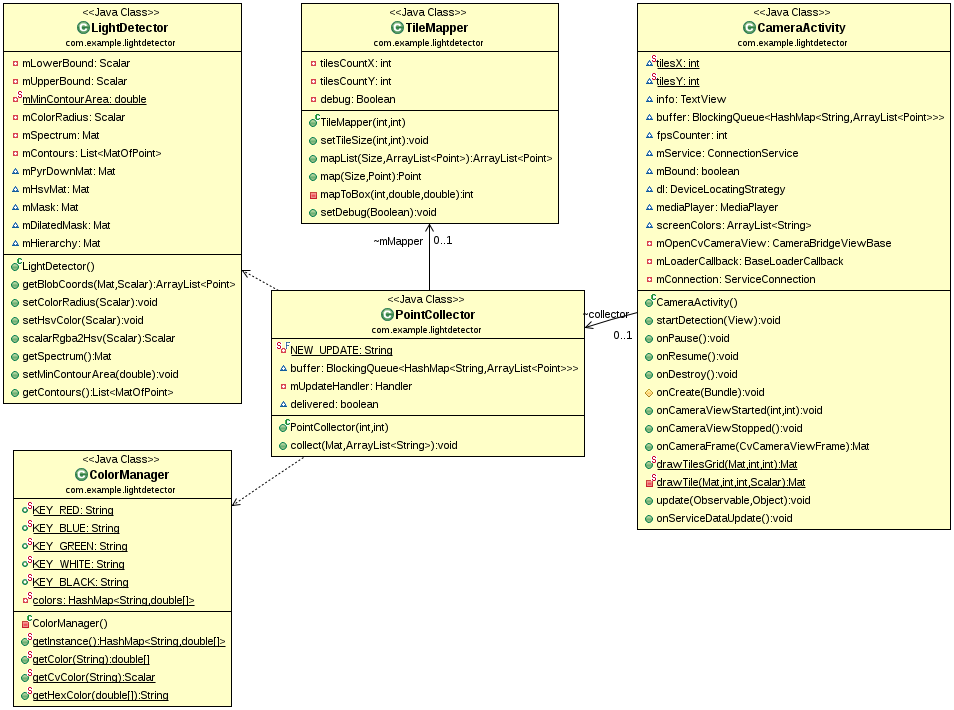
\includegraphics[width=16.2cm]{sprint3/sprint3.png}
	\caption{Sprint 3 light detection module class diagram}
	\label{fig:class_diagram_sprint3}
\end{figure}

\subsection{Physical view}


\begin{figure}[H]
	\centering
		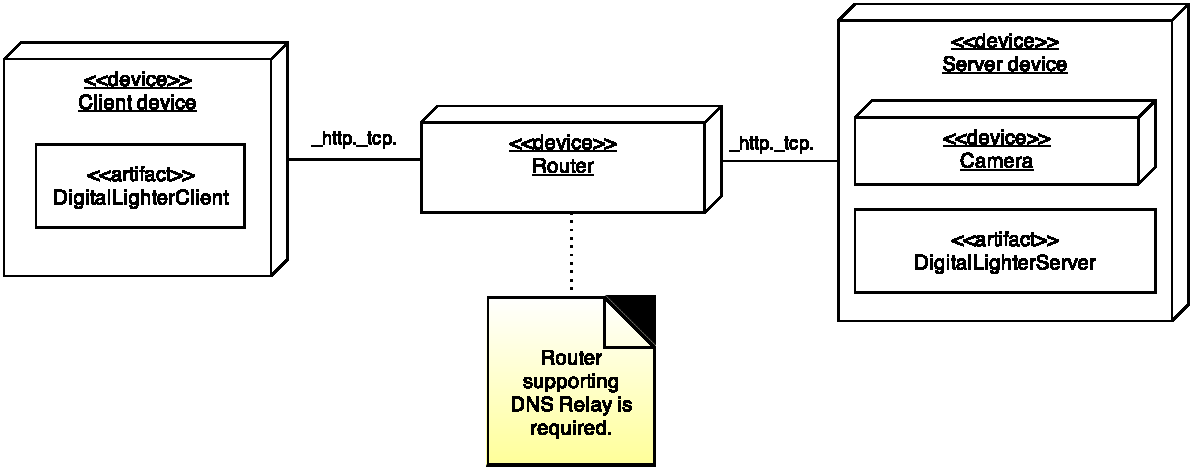
\includegraphics[width=15cm]{images/deployment-diagram-sprint3}
	\caption{Deployment diagram}
	\label{fig:sprint3_deployment_diagram}
\end{figure}

\subsection{Process view}
You can see the process view represented in Figures \ref{fig:sprint3_activity_diagram} and \ref{fig:sprint3_dfd}.
It should be mentioned, that each time new image was taken by camera, new thread is created and therefore several processing in the same time can be performed.

\begin{figure}[H]
	\centering
		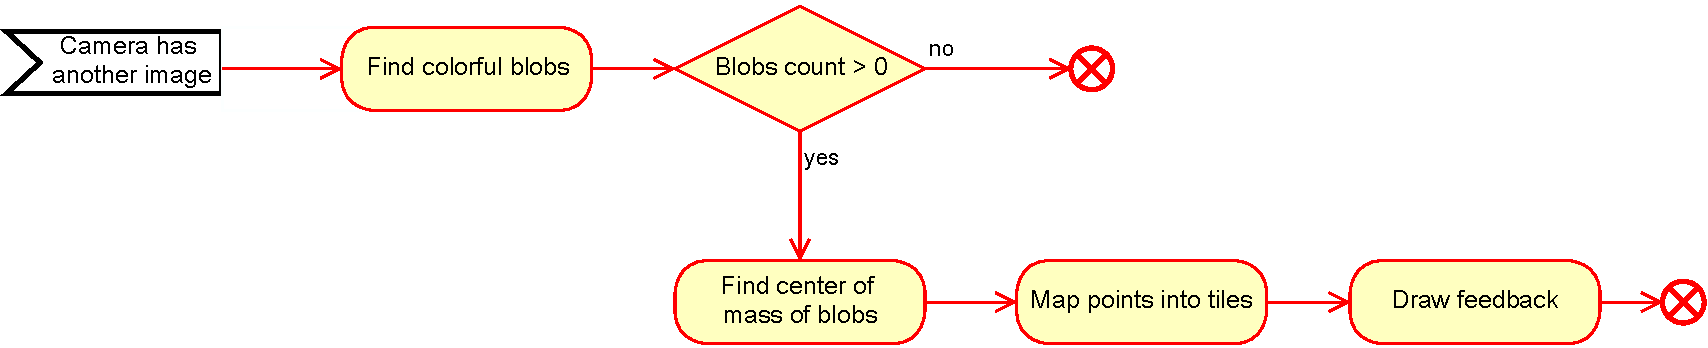
\includegraphics[width=16.2cm]{sprint3/sprint3_activity.pdf}
	\caption{Sprint 3 activity diagram}
	\label{fig:sprint3_activity_diagram}
\end{figure}


\begin{figure}[H]
	\centering
		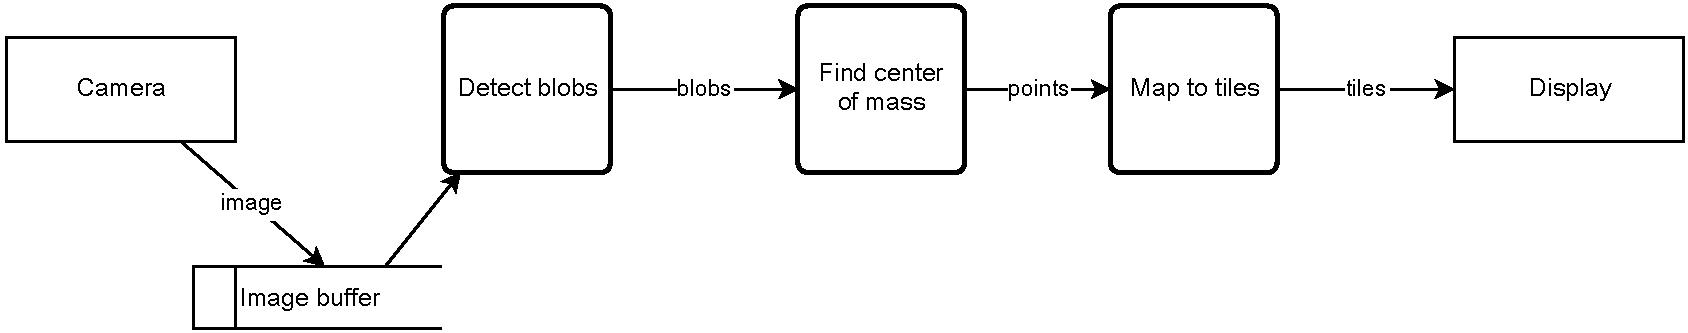
\includegraphics[width=16.2cm]{sprint3/sprint3_dtd.pdf}
	\caption{Sprint 3 data flow diagram}
	\label{fig:sprint3_dfd}
\end{figure}

%\subsection{Development view}
%Since this is a single module, there is no need for development view

\section{Implementation}

Few problems during implementation had occurred. 
Since the OpenCV library for Java is in early stage, there is some functionality missing.
One of these is a method \texttt{open(String)} of class \texttt{VideoCapture}\footnote{http://docs.opencv.org/java/org/opencv/highgui/VideoCapture.html}.
In C++ version of OpenCV there exist such a method and it programmers allows to use a video for input for image processing.
After short research, a fix of this bug was found\footnote{http://code.opencv.org/issues/3207}, but this feature will be added in release 2.4.7.


\section{Testing}


\section{Occurring risks}
\section{Retrospective}
\subsection{Pros}
\subsection{Cons}
\section{Evaluation}